\begin{frame}[t]{Translation of Light  - A Question of Marriage}
\begin{columns}[T, onlytextwidth]
\column{0.5\textwidth}
\Mercury\ (L1) (querent) \Quincunx\ \Jupiter\ (L7) (marriage) \\
\Moon\ separating \Sextile\ \Mercury\ applying \Square\ \Jupiter \\
\vspace{0.25cm}
Therefore, the \Moon\ was carrying the light of \Mercury\ to \Jupiter\ \textsl{"and this signified the completion of the thing, i.e. the attainment of the woman through the hands of go-betweens and those running back and forth between the two [parties]."} ([JH] p14-15) \\
\vspace{0.15cm}
\textbf{Note:} \\
\small
In this example, it would seem that the \Moon\ is  the querent's main significator as \Mercury\ does not aspect the 1st house. \\

\column{0.5\textwidth}
\begin{center}
{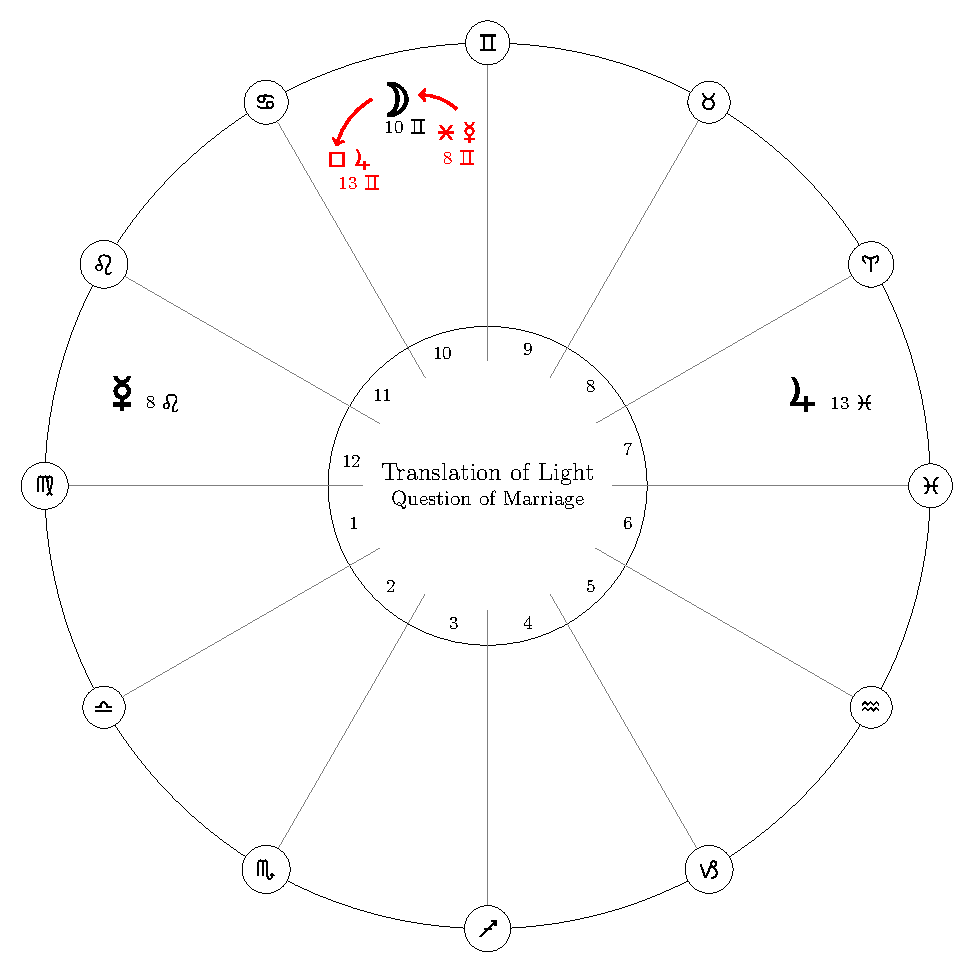
\includegraphics[width=0.9\textwidth]{charts/60-translation}} \\
\end{center}
\end{columns}
\end{frame}